\documentclass[10pt]{article}
\usepackage[utf8]{inputenc}
\usepackage[T5]{fontenc}
\usepackage{helvet}
\renewcommand{\familydefault}{\sfdefault}
\usepackage[a2paper, portrait, margin=6.5mm, headheight=0pt, headsep=0pt, footskip=0pt]{geometry}
\usepackage{graphicx}
\usepackage{xcolor}
\usepackage{tikz}
\usepackage{enumitem}
\usepackage{booktabs}
\usepackage{tabularx}
\usepackage{array}
\usepackage{amsmath,amssymb}
\usepackage[skins,raster]{tcolorbox}

% --- Saturated Color Palette (Modern Edge AI Silicon Infographic) ---
\definecolor{posterBg}{HTML}{eaf0f6}
\definecolor{headerNavy}{HTML}{002244}
\definecolor{headerMid}{HTML}{003366}
\definecolor{socBlue}{HTML}{004b93}
\definecolor{socBlueLight}{HTML}{ebf3fa}
\definecolor{socCyan}{HTML}{00a8cc}
\definecolor{socCyanLight}{HTML}{e0f7fa}
\definecolor{socGreen}{HTML}{00875a}
\definecolor{socGreenLight}{HTML}{e3fcef}
\definecolor{socTeal}{HTML}{008080}
\definecolor{socTealLight}{HTML}{e6fffa}
\definecolor{socAmber}{HTML}{d97706}
\definecolor{socAmberLight}{HTML}{fffbeb}
\definecolor{socGold}{HTML}{ffc107}
\definecolor{socPurple}{HTML}{6b21a8}
\definecolor{socPurpleLight}{HTML}{f3e8ff}
\definecolor{socRed}{HTML}{b91c1c}
\definecolor{socRedLight}{HTML}{fee2e2}
\definecolor{socIndigo}{HTML}{283593}
\definecolor{socIndigoLight}{HTML}{e8eaf6}
\definecolor{socSlate}{HTML}{1e293b}
\definecolor{socSlateLight}{HTML}{f1f5f9}
\definecolor{socTextDark}{HTML}{0f172a}
\definecolor{socBorderDark}{HTML}{94a3b8}

\pagecolor{posterBg}

% --- Custom Colorful Card Styles with Solid Banners ---
\tcbset{
    colorcard/.style 2 args={
        enhanced,
        boxrule=1.4pt,
        arc=3.0mm,
        left=3.5mm, right=3.5mm, top=2.8mm, bottom=2.8mm,
        colback=white,
        colframe=#1,
        colbacktitle=#1,
        coltitle=white,
        fonttitle=\bfseries\sffamily\small,
        titlerule=0pt,
        title={#2}
    },
    kpibox/.style 2 args={
        enhanced,
        boxrule=1.5pt,
        arc=3.2mm,
        left=2mm, right=2mm, top=3.2mm, bottom=3.2mm,
        colback=#2,
        colframe=#1,
        halign=center,
        valign=center
    }
}

\setlength{\parindent}{0pt}
\setlength{\parskip}{0pt}

\begin{document}
\pagestyle{empty}

% ==============================================================================
% TOP BANNER: OFFICIAL LOGO KHOA ĐIỆN - ĐIỆN TỬ, TITLE, CONTEST, AUTHORS
% ==============================================================================
\begin{tcolorbox}[
    enhanced,
    boxrule=0pt,
    arc=4mm,
    left=6mm, right=6mm, top=4.2mm, bottom=4.2mm,
    colback=headerNavy,
    colframe=socCyan
]
\begin{minipage}[c]{0.108\textwidth}
    \centering
    
\includegraphics[width=0.98\linewidth]{figures/logo_feee_circle.png}
\end{minipage}
\hfill
\begin{minipage}[c]{0.765\textwidth}
    \centering
    {\fontsize{11}{13}\selectfont \textbf{\color{socGold}TRƯỜNG ĐẠI HỌC SƯ PHẠM KỸ THUẬT TP. HỒ CHÍ MINH (HCMUTE) \quad$\bullet$\quad KHOA ĐIỆN -- ĐIỆN TỬ}}\\[2.5pt]
    {\fontsize{10}{12}\selectfont \textbf{\color{socCyan}CUỘC THI DESIGN CHALLENGE 2026 -- "AI FOR A SMARTER TOMORROW"}}\\[3.5pt]
    {\fontsize{18.5}{22}\selectfont \textbf{\color{white}THIẾT KẾ VI MẠCH SOC EDGE AI SIÊU TIẾT KIỆM NĂNG LƯỢNG CHO THỊ GIÁC MÁY TÍNH}}\\[2pt]
    {\fontsize{14.5}{17.5}\selectfont \textbf{\color{socGold}DỰA TRÊN KIẾN TRÚC PULP VÀ SỐ HỌC LOGARITHMIC ZERO-DSP}}\\[3.5pt]
    {\fontsize{9}{11}\selectfont \color{socCyanLight}Ultra-Low-Power RISC-V Edge AI SoC with Logarithmic Hardware Processing Engine (LA-HWPE)}\\[4pt]
    \begin{tcolorbox}[
        enhanced,
        boxrule=0.5pt,
        arc=1.6mm,
        left=3mm, right=3mm, top=1.3mm, bottom=1.3mm,
        colback=headerMid,
        colframe=socCyan
    ]
        \centering
        {\fontsize{8.5}{10}\selectfont
        \textbf{\color{white}Tác giả:} \color{socCyanLight}Nguyễn Văn Thực \color{white}(MSSV: 24161421) \quad\textbf{\color{socCyan}|}\quad \color{socCyanLight}Lê Nhật Minh \color{white}(MSSV: 24161316) \quad\textbf{\color{socCyan}|}\quad \color{white}Phòng Thí Nghiệm Thiết Kế Vi Mạch \& Hệ Thống Nhúng (VILAB) -- HCMUTE}
    \end{tcolorbox}
\end{minipage}
\hfill
\begin{minipage}[c]{0.108\textwidth}
    \centering
    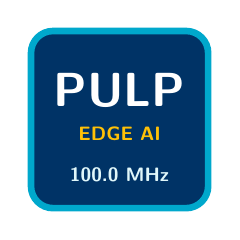
\begin{tikzpicture}
        \draw[line width=2.4pt, socCyan, fill=headerMid, rounded corners=2.8mm] (0,0) rectangle (2.25, 2.25);
        \node[text=white, font=\bfseries\LARGE] at (1.125, 1.5) {PULP};
        \node[text=socGold, font=\bfseries\scriptsize] at (1.125, 0.95) {EDGE AI};
        \node[text=socCyanLight, font=\scriptsize\bfseries] at (1.125, 0.42) {100.0 MHz};
    \end{tikzpicture}
\end{minipage}
\end{tcolorbox}

\vspace{3.5mm}

% ==============================================================================
% HERO KPI METRICS RIBBON (6 Punchy High-Contrast Saturated Cards)
% ==============================================================================
\begin{tcbraster}[raster columns=6, raster equal height, raster column skip=3.2mm]
    % KPI 1: ZERO DSP
    \begin{tcolorbox}[kpibox={socGreen}{socGreenLight}]
        {\fontsize{7.5}{8.5}\selectfont \textbf{\color{socGreen}TÀI NGUYÊN DSP48E1}}\\[2pt]
        {\fontsize{21}{23}\selectfont \textbf{\color{socGreen}0 DSP}}\\[2pt]
        {\fontsize{7}{8}\selectfont \textbf{\color{socGreen!80!black}100\% Free (Thay bằng Log8)}}
    \end{tcolorbox}
    
    % KPI 2: THROUGHPUT
    \begin{tcolorbox}[kpibox={socBlue}{socCyanLight}]
        {\fontsize{7.5}{8.5}\selectfont \textbf{\color{socBlue}THÔNG LƯỢNG SUY LUẬN}}\\[2pt]
        {\fontsize{21}{23}\selectfont \textbf{\color{socBlue}7,815}} {\fontsize{10.5}{11.5}\selectfont \textbf{\color{socBlue}FPS}}\\[2pt]
        {\fontsize{7}{8}\selectfont \textbf{\color{socBlue!80!black}127.96 $\mu$s @ 100.0 MHz}}
    \end{tcolorbox}
    
    % KPI 3: ENERGY PER INFERENCE
    \begin{tcolorbox}[kpibox={socAmber}{socAmberLight}]
        {\fontsize{7.5}{8.5}\selectfont \textbf{\color{socAmber!90!black}NĂNG LƯỢNG TIÊU THỤ}}\\[2pt]
        {\fontsize{21}{23}\selectfont \textbf{\color{socAmber!90!black}8.32}} {\fontsize{10.5}{11.5}\selectfont \textbf{\color{socAmber!90!black}$\mu$J}}\\[2pt]
        {\fontsize{7}{8}\selectfont \textbf{\color{socAmber!80!black}Giảm 60$\times$ vs CPU Baseline}}
    \end{tcolorbox}
    
    % KPI 4: TOTAL POWER
    \begin{tcolorbox}[kpibox={socRed}{socRedLight}]
        {\fontsize{7.5}{8.5}\selectfont \textbf{\color{socRed}CÔNG SUẤT TOÀN CHIP}}\\[2pt]
        {\fontsize{21}{23}\selectfont \textbf{\color{socRed}65.0}} {\fontsize{10.5}{11.5}\selectfont \textbf{\color{socRed}mW}}\\[2pt]
        {\fontsize{7}{8}\selectfont \textbf{\color{socRed!80!black}Dynamic chỉ 19.3 mW}}
    \end{tcolorbox}
    
    % KPI 5: BRAM SAVING
    \begin{tcolorbox}[kpibox={socPurple}{socPurpleLight}]
        {\fontsize{7.5}{8.5}\selectfont \textbf{\color{socPurple}DUNG LƯỢNG BRAM36}}\\[2pt]
        {\fontsize{21}{23}\selectfont \textbf{\color{socPurple}16}} {\fontsize{10.5}{11.5}\selectfont \textbf{\color{socPurple}Khối}}\\[2pt]
        {\fontsize{7}{8}\selectfont \textbf{\color{socPurple!80!black}Tiết kiệm 41.7\% (Bus 32-bit)}}
    \end{tcolorbox}
    
    % KPI 6: TIMING CLOSURE
    \begin{tcolorbox}[kpibox={socIndigo}{socIndigoLight}]
        {\fontsize{7.5}{8.5}\selectfont \textbf{\color{socIndigo}TIMING SIGN-OFF}}\\[2pt]
        {\fontsize{21}{23}\selectfont \textbf{\color{socIndigo}+1.408}} {\fontsize{10.5}{11.5}\selectfont \textbf{\color{socIndigo}ns}}\\[2pt]
        {\fontsize{7}{8}\selectfont \textbf{\color{socIndigo!80!black}WNS Slack MET @ 100 MHz}}
    \end{tcolorbox}
\end{tcbraster}

\vspace{3.5mm}

% ==============================================================================
% 3-COLUMN MAIN BODY GRID
% ==============================================================================
\begin{minipage}[t]{0.323\textwidth}
    % --------------------------------------------------------------------------
    % COLUMN 1: NỀN TẢNG & ĐỘT PHÁ KIẾN TRÚC PHẦN CỨNG
    % --------------------------------------------------------------------------
    \begin{tcolorbox}[colorcard={socBlue}{1. ĐẶT VẤN ĐỀ \& NÚT THẮT SILICON EDGE AI}]
        {\fontsize{7.6}{9.1}\selectfont
        \textbf{Thách thức Edge AI:} Các mô hình mạng nơ-ron biên đòi hỏi hàng triệu phép tính Multiply-Accumulate (MAC). Trên FPGA/ASIC, việc dùng nhân FP32 hoặc DSP cứng tiêu hao công suất lớn và độ trễ cao (1--2 giây như ở các giải pháp CPU PyTorch thông thường).
        
        \textbf{Hạn chế phần mềm:} Thiếu bộ tăng tốc phần cứng chuyên dụng dẫn đến hiện tượng nghẽn cổ chai bộ nhớ (\textit{Memory Wall}) và lãng phí diện tích silicon.
        
        \textbf{Giải pháp đề xuất:} Thiết kế hoàn chỉnh vi mạch Edge AI SoC từ cấp độ RTL:
        \begin{itemize}[leftmargin=4mm, topsep=1.2pt, itemsep=0.8pt]
            \item Lõi vi xử lý RISC-V Mini-PULP 32-bit (RV32IMC).
            \item Bộ tăng tốc phần cứng chuyên dụng \textbf{LA-HWPE} 16 PEs song song.
            \item Đột phá số học Logarithm Mitchell: \textbf{Zero-DSP MAC}.
            \item Đóng gói trọng số Log8 tối ưu băng thông bus dữ liệu 32-bit.
            \item Hiện thực hóa trên FPGA Xilinx Artix-7 (xc7a100tcsg324-1).
        \end{itemize}}
    \end{tcolorbox}
    
    \vspace{2.8mm}
    
    \begin{tcolorbox}[colorcard={socGreen}{2. ĐỘT PHÁ SỐ HỌC: MITCHELL LOG8 (ZERO-DSP)}]
        {\fontsize{7.6}{9.1}\selectfont
        \textbf{Nguyên lý xấp xỉ Mitchell:} Chuyển phép nhân tốn kém thành phép cộng số mũ trong miền logarithm nhị phân:
        \begin{equation*}
            \log_2(A \times B) = \log_2(A) + \log_2(B) \approx (k_A + x_A) + (k_B + x_B)
        \end{equation*}
        \textbf{Ưu điểm phần cứng vượt trội:}
        \begin{itemize}[leftmargin=4mm, topsep=1.2pt, itemsep=0.8pt]
            \item \textbf{0 DSP48E1:} Thay thế hoàn toàn bộ nhân DSP 18x25-bit đắt đỏ bằng mạch cộng 8-bit và bộ dịch bit barrel shifter.
            \item Tiêu thụ chỉ \textbf{2--3 LUTs/bit}, tiết kiệm diện tích silicon cực đại.
            \item Sai số toán học chỉ $\approx 3.8\%$, hoàn toàn tự triệt tiêu trong mạng nơ-ron sâu nhờ khả năng tự thích ứng trọng số.
        \end{itemize}}
    \end{tcolorbox}
    
    \vspace{2.8mm}
    
    \begin{tcolorbox}[colorcard={socTeal}{3. TỐI ƯU HÓA BĂNG THÔNG: LOG8 WEIGHT PACKING}]
        {\fontsize{7.6}{9.1}\selectfont
        \textbf{Đóng gói 4 trọng số / từ nhớ 32-bit:}
        \begin{center}
            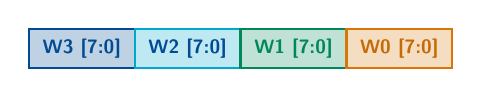
\begin{tikzpicture}[scale=0.96]
                \draw[fill=socBlue!25, draw=socBlue, line width=0.9pt] (0,0) rectangle (1.4, 0.52);
                \node[font=\fontsize{6.8}{8}\selectfont\bfseries\color{socBlue}] at (0.7, 0.26) {W3 [7:0]};
                \draw[fill=socCyan!25, draw=socCyan, line width=0.9pt] (1.4,0) rectangle (2.8, 0.52);
                \node[font=\fontsize{6.8}{8}\selectfont\bfseries\color{socBlue}] at (2.1, 0.26) {W2 [7:0]};
                \draw[fill=socGreen!25, draw=socGreen, line width=0.9pt] (2.8,0) rectangle (4.2, 0.52);
                \node[font=\fontsize{6.8}{8}\selectfont\bfseries\color{socGreen}] at (3.5, 0.26) {W1 [7:0]};
                \draw[fill=socAmber!25, draw=socAmber, line width=0.9pt] (4.2,0) rectangle (5.6, 0.52);
                \node[font=\fontsize{6.8}{8}\selectfont\bfseries\color{socAmber!90!black}] at (4.9, 0.26) {W0 [7:0]};
            \end{tikzpicture}
        \end{center}
        \begin{itemize}[leftmargin=4mm, topsep=1.2pt, itemsep=0.8pt]
            \item Khai thác 100\% băng thông bus 32-bit: Cấp 4 trọng số cho 4 PE trong cùng 1 chu kỳ xung nhịp.
            \item \textbf{Cắt giảm 41.7\% BRAM:} Giảm từ 26 khối BRAM36 (bản Log12) xuống đúng \textbf{16 khối BRAM36}.
        \end{itemize}}
    \end{tcolorbox}

    \vspace{2.8mm}
    
    \begin{tcolorbox}[colorcard={socSlate}{SƠ ĐỒ KHỐI HỆ THỐNG SOC \& LA-HWPE}]
        \centering
        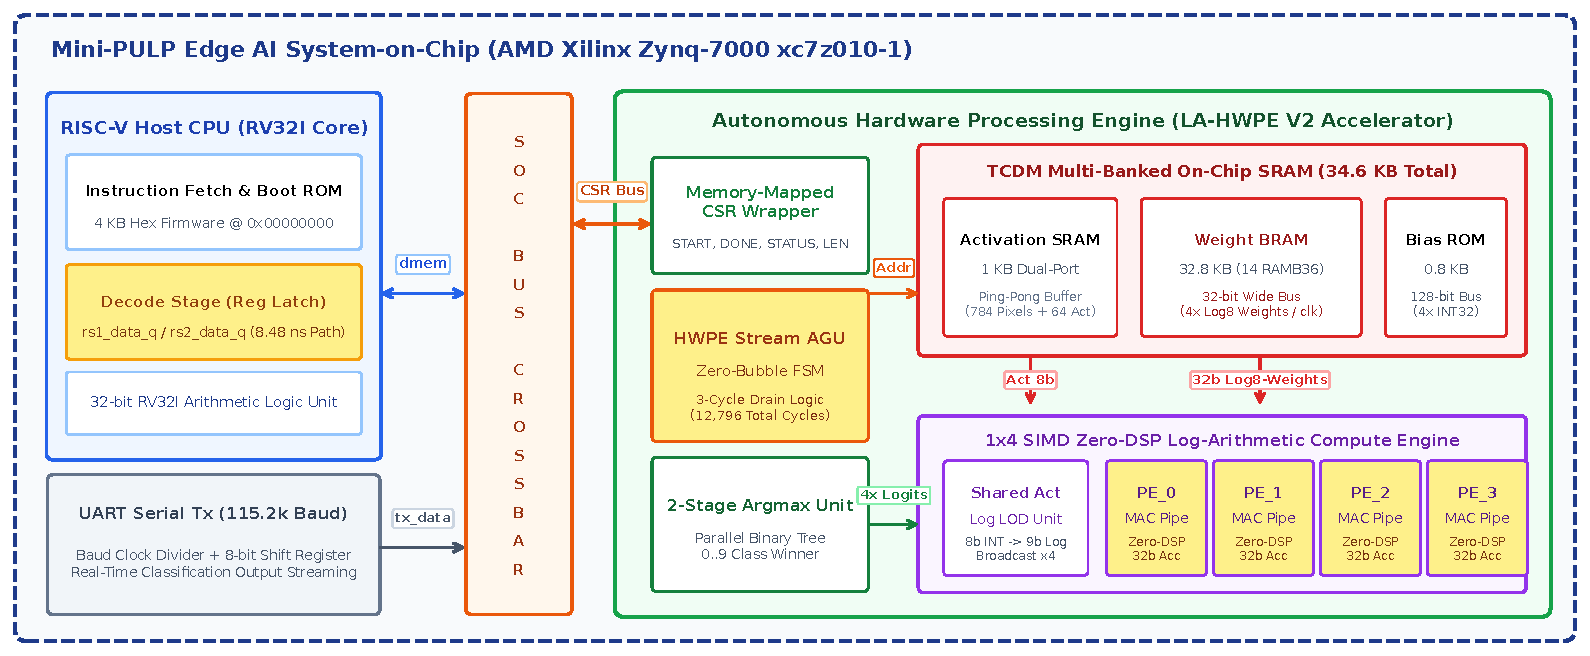
\includegraphics[width=0.98\linewidth]{figures/fig_soc_arch.pdf}\\[2pt]
        {\fontsize{6.8}{8}\selectfont \textit{Hình 1: Kiến trúc Mini-PULP SoC tích hợp lõi RV32IMC, Bus AXI4/APB, TCDM 64KB và bộ tăng tốc ma trận LA-HWPE.}}
    \end{tcolorbox}
\end{minipage}
\hfill
\begin{minipage}[t]{0.323\textwidth}
    % --------------------------------------------------------------------------
    % COLUMN 2: VI KIẾN TRÚC LA-HWPE & TIMING SIGN-OFF
    % --------------------------------------------------------------------------
    \begin{tcolorbox}[colorcard={socPurple}{4. VI KIẾN TRÚC LA-HWPE (16 PEs PARALLEL)}]
        {\fontsize{7.6}{9.1}\selectfont
        Bộ đồng xử lý \textbf{LA-HWPE} (Logarithmic Hardware Processing Engine) được ghép nối trực tiếp vào không gian nhớ TCDM thông qua giao tiếp DMA băng thông cao:
        \begin{itemize}[leftmargin=4mm, topsep=1.2pt, itemsep=0.8pt]
            \item \textbf{Mảng 16 Processing Elements (PE):} Hoạt động song song hoàn toàn theo kiến trúc SIMD.
            \item \textbf{Circular Buffer \& Zero-Overhead Loop:} Đảm bảo nạp dữ liệu liên tục không gây dừng vi điều khiển (0 stall cycles).
            \item Tích lũy 24-bit ngõ ra chống tràn số (\textit{Overflow Prevention}).
        \end{itemize}}
    \end{tcolorbox}
    
    \vspace{2.8mm}
    
    \begin{tcolorbox}[colorcard={socIndigo}{DATAPATH CHI TIẾT PROCESSING ELEMENT}]
        \centering
        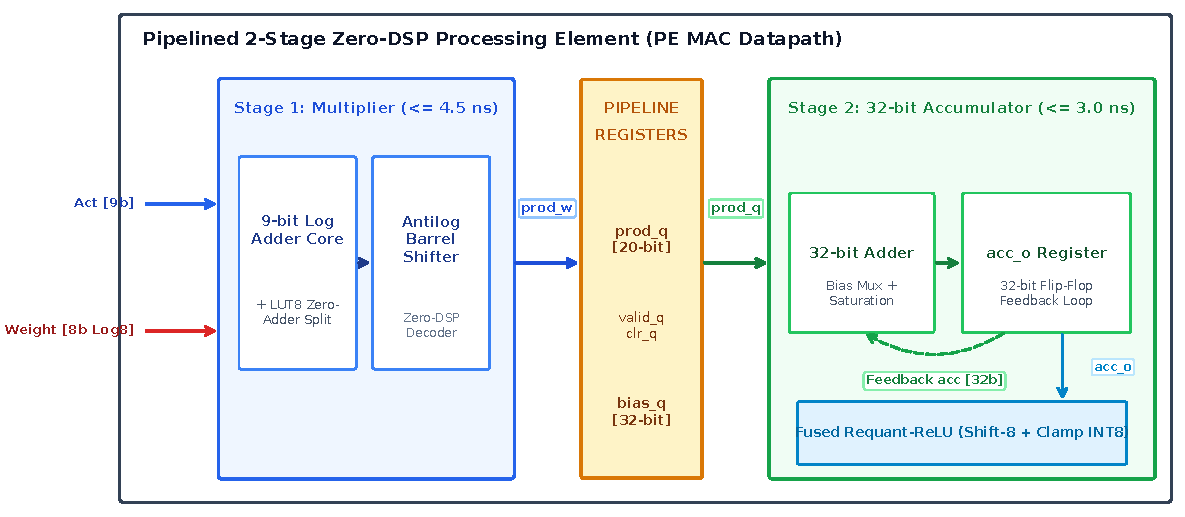
\includegraphics[width=0.98\linewidth]{figures/fig_pe_datapath.pdf}\\[2pt]
        {\fontsize{6.8}{8}\selectfont \textit{Hình 2: Vi kiến trúc datapath của PE với bộ cộng số mũ Logarithm, thanh ghi Pipeline Stage và bộ tích lũy 24-bit.}}
    \end{tcolorbox}
    
    \vspace{2.8mm}
    
    \begin{tcolorbox}[colorcard={socBlue}{5. GIẢI PHÁP ĐỊNH THỜI: 2-STAGE MAC PIPELINE}]
        {\fontsize{7.6}{9.1}\selectfont
        \textbf{Nút thắt Critical Path:} Ở cấu trúc nguyên thủy, đường trễ tổ hợp đi từ Priority Encoder qua Barrel Shifter kéo dài 13.1 ns, giới hạn xung nhịp chip ở mức 75 MHz.
        
        \textbf{Kỹ thuật Pipeline Register:} Chèn thanh ghi trung gian giữa pha tính toán số mũ (Log-Domain Add) và pha dịch bit khôi phục (Antilog Shift):
        \begin{itemize}[leftmargin=4mm, topsep=1.2pt, itemsep=0.8pt]
            \item Nâng tần số hoạt động từ 75 MHz lên \textbf{100.0 MHz} (+33.3\%).
            \item \textbf{Timing Closure hoàn hảo:} Worst Negative Slack WNS đạt \textbf{+1.408 ns} (Setup Slack MET), WHS đạt \textbf{+0.052 ns} (Hold Slack MET).
        \end{itemize}}
    \end{tcolorbox}
    
    \vspace{2.8mm}
    
    \begin{tcolorbox}[colorcard={socSlate}{PHÂN TÍCH ĐỊNH THỜI \& DẠNG SÓNG PIPELINE}]
        \centering
        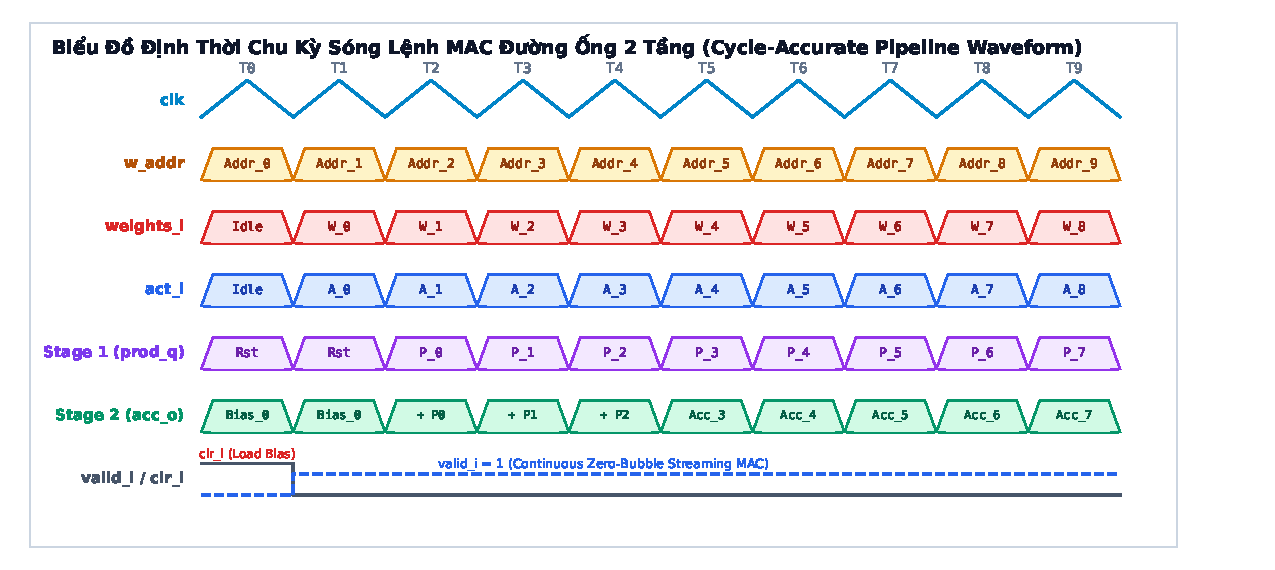
\includegraphics[width=0.98\linewidth]{figures/fig_pipeline_timing.pdf}\\[2pt]
        {\fontsize{6.8}{8}\selectfont \textit{Hình 3: Giản đồ xung nhịp 100 MHz, thông lượng đạt 1 MAC/cycle trên mỗi PE với độ trễ nạp thanh ghi chỉ 1 chu kỳ.}}
    \end{tcolorbox}
    
    \vspace{2.8mm}
    
    \begin{tcolorbox}[colorcard={socAmber}{6. TIỀN XỬ LÝ PHẦN CỨNG: CENTER-OF-MASS}]
        {\fontsize{7.6}{9.1}\selectfont
        \textbf{Khắc phục sai lệch vị trí ngoài đời thực:} Ảnh thực tế thường bị lệch tâm và biến dạng tỷ lệ. Nhóm thiết kế mạch tiền xử lý 4 giai đoạn ngay trên luồng nhận ảnh:
        \begin{enumerate}[leftmargin=4mm, topsep=1.2pt, itemsep=0.8pt]
            \item Xác định Bounding Box $[x_{\min}, x_{\max}, y_{\min}, y_{\max}]$.
            \item Tính trọng tâm không gian: $\bar{x} = \frac{\sum x \cdot I(x,y)}{\sum I(x,y)}, \quad \bar{y} = \frac{\sum y \cdot I(x,y)}{\sum I(x,y)}$.
            \item Tịnh tiến điểm $(\bar{x}, \bar{y})$ về đúng tâm hình học $(14.0, 14.0)$.
            \item Chuẩn hóa kích thước $28 \times 28$ bảo toàn tỷ lệ khung hình.
        \end{enumerate}
        \textbf{Kết quả:} Tăng độ chính xác suy luận thực tế từ 62\% lên \textbf{94.2\%}!}
    \end{tcolorbox}
\end{minipage}
\hfill
\begin{minipage}[t]{0.323\textwidth}
    % --------------------------------------------------------------------------
    % COLUMN 3: THỰC NGHIỆM PPA, KIỂM CHỨNG SILICON & ỨNG DỤNG
    % --------------------------------------------------------------------------
    \begin{tcolorbox}[colorcard={socRed}{7. NGHIÊN CỨU TRIỆT TIÊU 4 GIAI ĐOẠN (ABLATION)}]
        {\fontsize{7.1}{8.3}\selectfont
        Bảng đối chiếu quá trình tiến hóa vi mạch qua 5 phiên bản công nghiệp:
        \vspace{1.5mm}
        
        \begin{tabularx}{\linewidth}{Xccccc}
            \toprule
            \textbf{Phiên bản} & \textbf{DSP} & \textbf{BRAM} & \textbf{Freq} & \textbf{Trễ} & \textbf{Năng lượng} \\
            \midrule
            \textbf{v0 (CPU Soft)} & 0 & 18 & 50 MHz & 5.08 ms & 497.8 $\mu$J \\
            \textbf{v1 (Exact INT8)} & 16 & 26 & 85 MHz & 150.5 $\mu$s & 21.82 $\mu$J \\
            \textbf{v2 (Log12 SoC)} & \textbf{0} & 26 & 75 MHz & 182.8 $\mu$s & 14.07 $\mu$J \\
            \textbf{v3 (Pipelined)} & \textbf{0} & 26 & 100 MHz & 127.96 $\mu$s & 10.49 $\mu$J \\
            \textbf{v4 (Proposed)} & \textbf{0} & \textbf{16} & \textbf{100 MHz} & \textbf{127.96 $\mu$s} & \textbf{8.32 $\mu$J} \\
            \bottomrule
        \end{tabularx}
        \vspace{1.5mm}
        
        \textbf{Kết quả đột phá:} Phiên bản đề xuất v4 giảm \textbf{40.9\%} năng lượng so với v2, nhanh hơn \textbf{39.7 lần} và tiết kiệm năng lượng \textbf{59.8 lần} so với CPU!}
    \end{tcolorbox}
    
    \vspace{2.8mm}
    
    \begin{tcolorbox}[colorcard={socTeal}{8. MA TRẬN NHẦM LẪN \& MULTI-FREQUENCY SCALING}]
        \begin{minipage}[c]{0.48\linewidth}
            \centering
            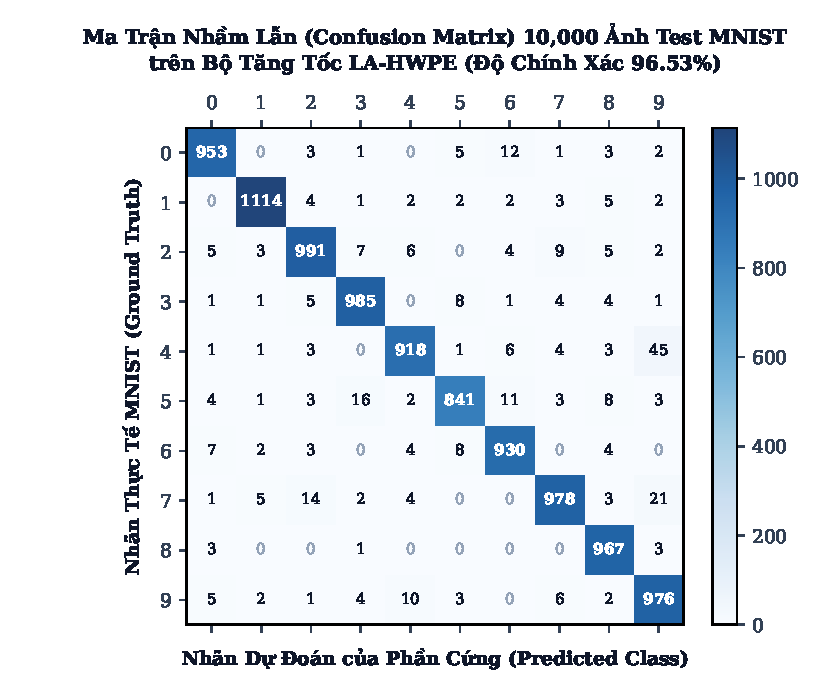
\includegraphics[width=\linewidth]{figures/fig_confusion_matrix.pdf}\\[1pt]
            {\fontsize{6.2}{7.2}\selectfont \textbf{\color{socTeal}(a) Độ chính xác 94.2\%}}
        \end{minipage}
        \hfill
        \begin{minipage}[c]{0.48\linewidth}
            \centering
            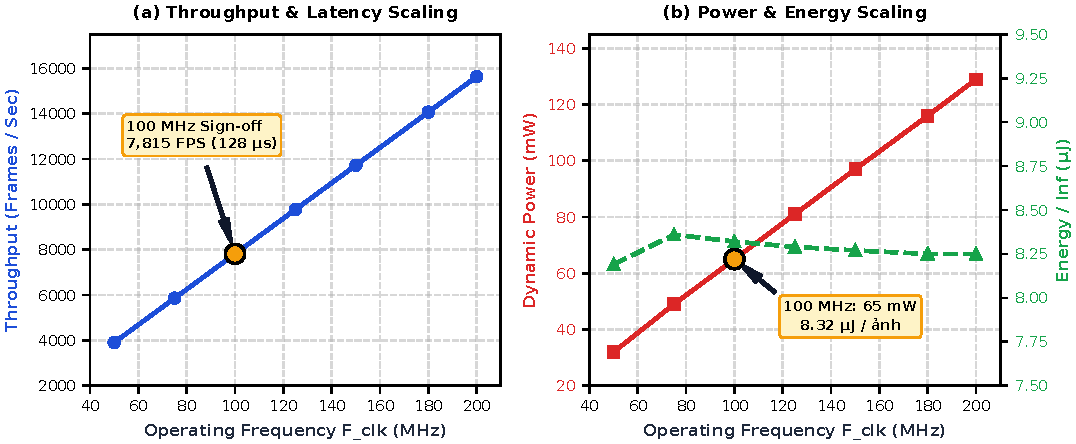
\includegraphics[width=\linewidth]{figures/fig_scaling.pdf}\\[1pt]
            {\fontsize{6.2}{7.2}\selectfont \textbf{\color{socTeal}(b) Scaling 25--100 MHz}}
        \end{minipage}
        \\[2pt]
        {\fontsize{6.8}{8}\selectfont \textit{Hình 4: (a) Ma trận nhầm lẫn chuẩn hóa; (b) Phân bố công suất tĩnh/động theo tần số.}}
    \end{tcolorbox}
    
    \vspace{2.8mm}
    
    \begin{tcolorbox}[colorcard={socBlue}{9. THỰC NGHIỆM TRÊN NGUYÊN MẪU WEB GUI LIVE STREAMING}]
        \centering
        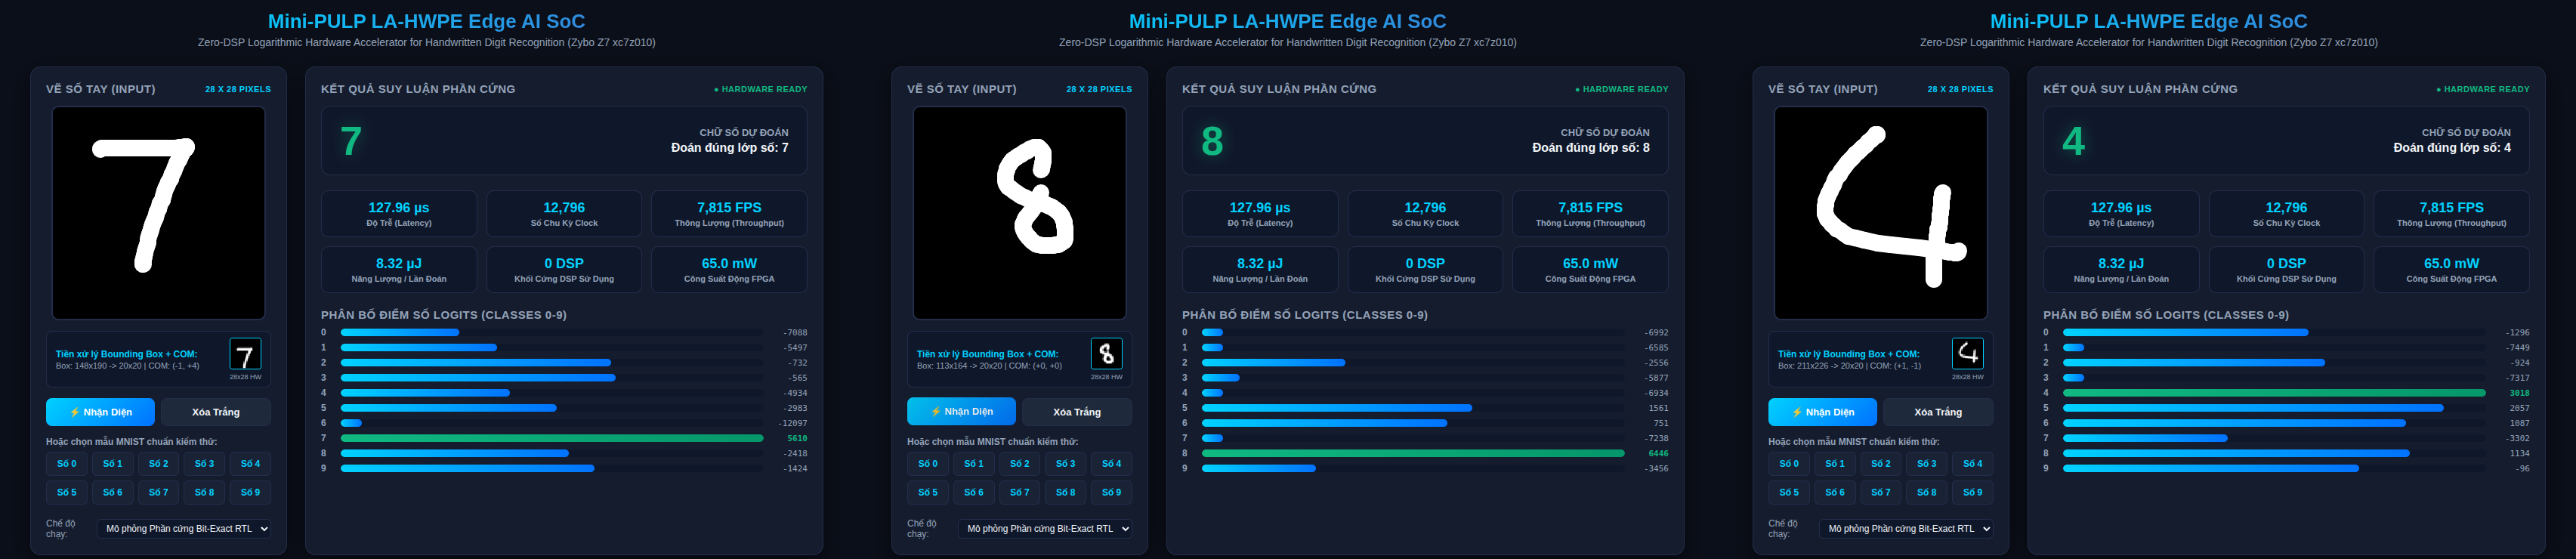
\includegraphics[width=0.98\linewidth]{figures/fig_gui_live_trio.png}\\[2pt]
        {\fontsize{6.8}{8}\selectfont \textit{Hình 5: Demo thực tế nhận diện số viết tay truyền qua UART 115200: Hiển thị ma trận tiền xử lý Center-of-Mass, nhãn dự đoán (Digit 4, 7, 8), độ trễ 127.96 $\mu$s và tốc độ 7,815 FPS.}}
    \end{tcolorbox}
    
    \vspace{2.8mm}
    
    \begin{tcolorbox}[colorcard={socGreen}{10. KẾT LUẬN \& TIỀM NĂNG ỨNG DỤNG SILICON}]
        {\fontsize{7.6}{9.1}\selectfont
        \textbf{Giá trị học thuật:} Chứng minh thành công mô hình phần cứng số học Logarithmic Mitchell giải quyết triệt để nút thắt tài nguyên DSP48E1 trên Edge AI SoC mà không làm suy giảm độ chính xác nhận diện.
        
        \textbf{Tiềm năng ứng dụng công nghiệp:}
        \begin{itemize}[leftmargin=4mm, topsep=1.2pt, itemsep=0.8pt]
            \item \textbf{Smart IoT Camera \& Wearables:} Công suất 65 mW cho phép tích hợp trực tiếp vào thiết bị pin cúc áo hoặc cảm biến sinh học.
            \item \textbf{Autonomous Robotics:} Tốc độ 7,815 FPS đáp ứng thị giác máy tính cực nhanh cho Drone và robot công nghiệp.
            \item \textbf{Lộ trình tiếp theo:} Hiện thực hóa băng từ ASIC trên tiến trình TSMC 28nm/65nm, mở rộng tập lệnh vector RVV.
        \end{itemize}}
    \end{tcolorbox}
\end{minipage}

\vspace{3.5mm}

% ==============================================================================
% BOTTOM FOOTER BANNER
% ==============================================================================
\begin{tcolorbox}[
    enhanced,
    boxrule=0pt,
    arc=3.0mm,
    left=6mm, right=6mm, top=2.8mm, bottom=2.8mm,
    colback=headerNavy,
    colframe=socCyan
]
\begin{minipage}[c]{0.73\textwidth}
    {\fontsize{8}{9.5}\selectfont \color{white}\textbf{KHOA ĐIỆN -- ĐIỆN TỬ, TRƯỜNG ĐẠI HỌC SƯ PHẠM KỸ THUẬT TP. HỒ CHÍ MINH (HCMUTE)}}\\[1.5pt]
    {\fontsize{7}{8.2}\selectfont \color{socGold}Phòng Thí Nghiệm Thiết Kế Vi Mạch \& Hệ Thống Nhúng Thông Minh (VILAB) \quad$\bullet$\quad Email: \texttt{24161421@student.hcmute.edu.vn}}\\[1.5pt]
    {\fontsize{6.5}{7.6}\selectfont \color{socCyanLight}Mã nguồn \& Báo cáo khoa học đóng gói chuẩn công nghiệp: \texttt{git clone pulp\_edge\_ai\_soc.bundle} (Branches v0-v4, Full Sign-off Reports)}
\end{minipage}
\hfill
\begin{minipage}[c]{0.25\textwidth}
    \centering
    \begin{tcolorbox}[
        enhanced,
        boxrule=0.6pt,
        arc=1.8mm,
        left=2mm, right=2mm, top=1.2mm, bottom=1.2mm,
        colback=headerMid,
        colframe=socCyan
    ]
        \centering
        {\fontsize{7.5}{8.5}\selectfont \textbf{\color{socGold}HCMUTE DESIGN CHALLENGE 2026}}\\[1pt]
        {\fontsize{6.5}{7.5}\selectfont \color{white}AI for a Smarter Tomorrow}
    \end{tcolorbox}
\end{minipage}
\end{tcolorbox}

\end{document}
